\documentclass{article}
\usepackage[utf8]{inputenc}
\usepackage{amsfonts}
\usepackage{algorithm2e}
\usepackage{amsmath}
\usepackage[a4paper]{geometry}
\geometry{hscale=0.8,vscale=0.9,centering}
\usepackage{graphicx}
\usepackage{program}
\usepackage{ulem}
\usepackage{xcolor}
\usepackage{pdfpages}
\usepackage{hyperref}
\newcommand{\subsubsubsection}[1]{\paragraph{#1}\mbox{}\\}
\setcounter{secnumdepth}{4}
\setcounter{tocdepth}{4}
\newcommand{\alinea}{
\textbf{\hspace{8mm}}
}
 \setlength{\parindent}{0pt}
 
\newcommand{\sautligne}{
\textbf{\vspace{5mm}}
}
\usepackage{pdflscape}
\newenvironment{changemargin}[2]{%
\begin{list}{}{%
\setlength{\topsep}{0pt}%
\setlength{\leftmargin}{#1}%
\setlength{\rightmargin}{#2}%
\setlength{\listparindent}{\parindent}%
\setlength{\itemindent}{\parindent}%
\setlength{\parsep}{\parskip}%
}%
\item[]}{\end{list}}


\title{M1 Info – ARC - LAB6}
\author{Olivier HUREAU - Groupe 3}
\date{21/04/2020}

\begin{document}
\maketitle
\renewcommand{\contentsname}{Table des matières}
\tableofcontents
\newpage


\newpage
\subsection{Conclusion}
La différence avec un codage de gray ou binaire n'est pas très significative. On as la même nombre de composants mémorisants mais le chemin critique est plus long pour le codage binaire.
\sautligne

Cependant avec un codage OneHot la fréquence est moitié plus grande qu'en binaire ou gray. La surface est un quart plus grande car utilise plus de composants mémorisant (DFC1 et DFP1)
\sautligne

On pouvais s'y attendre car le oneHot nécessite moins d'utilisation de composant mémorisant et c'est ceux la qui prennent le plus de temps.

En effet, plus le délai du chemin critique est faible, plus il sera possible de passer par celui la en une seconde. Donc la fréquence augmente.
\begin{landscape}
\newpage
\section{Simulation}
Pour analyser les différentes synthèse et le composant inital on vas alors regarder si la valeur des états est la même pour tout les composants et si les sorties sont toutes équivalentes.

les sorties devant être équivalentes sont alors : search, rest et food.

Ce qu'on vérifie ici :

\begin{figure}[!h]
\centering
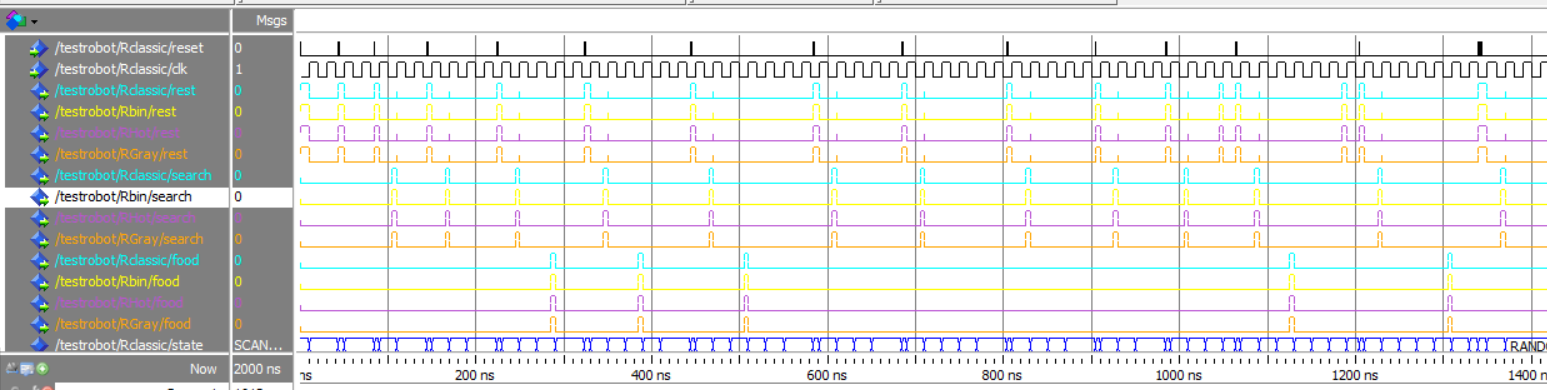
\includegraphics[scale=0.6]{C/OUTPUT_OK.PNG}
\caption{Chronograme avec les différentes valeurs de sorties }
\end{figure} 


On vérifie en suite pour les états.
On rappel les valeurs associés à chaque état.
\begin{figure}[!h]
\centering
\begin{tabular}{c | c | c | c}
	
	Etats & Binaire  & Gray  & OneHot   \\
\hline	
   IDLE & 0000 & 0000 &    000000010\\
   RESTING & -001 & 0001 & 000000100 \\
   RANDOMWALK & -010 & 0011 &  000000100 \\
   SCANAREA & -011 & 0010 & 000001000 \\
   HOMING & -100 &0110   & 000010000 \\ 
   MOVETOFOOD & -101&0111 &000100000 \\
   MOVETOHOME & -110 &0101&001000000 \\
   DEPOSIT & -111 & 0100 & 010000000 \\
   GRABFOOD & 1000& 1100  &100000000\\   
 \end{tabular}

\end{figure} 

Il est asses simple de retrouver ces valeurs pour la synthèse en Gray et la synthèse en Binaire car il existe les signaux correspondant : state\_0; state\_1; state\_2 ; state\_3.

Néanmoins pour la synthèse en OneHot il nous manque les signaux state\_6 et state\_8. Cela dois surement être du à une optimisation est que celui-ci n'était pas nécessaire. 

Cependant si l'on regarde le code VHDL de la synthèse. Chaque signaux correspond à un process. 

Par exemple : 

\begin{verbatim}
reg_state_2 : DFC1 port map ( Q=>state_2, QN=>OPEN, C=>clk, D=>nx64, RN=>nx759);
\end{verbatim}

Le signal state\_2 est modifié à la sortie du flip flop dans le process reg\_state\_2.

Si on s'intéresse au process reg\_state\_6 : 

\begin{verbatim}
reg_state_6 : DFC1 port map ( Q=>OPEN, QN=>nx767, C=>clk, D=>nx110, RN=>
\end{verbatim}

Rien n'est branché sur Q du flip flop mais on peut récupérer la valeur de state\_6 car c'est l'inverse de QN. On s'intéressera alors ç l'inverse du signal nx767.
\sautligne

Pareil pour state\_8 :
\begin{verbatim}
reg_state_8 : DFC1 port map ( Q=>OPEN, QN=>nx772, C=>clk, D=>nx102, RN=>
\end{verbatim}

Donc on surveillera nx772.

On vérifie alors que les valeurs des différents signaux coincident bien avec les états courants sur le chronogramme suivant :

\begin{figure}[!h]
\centering
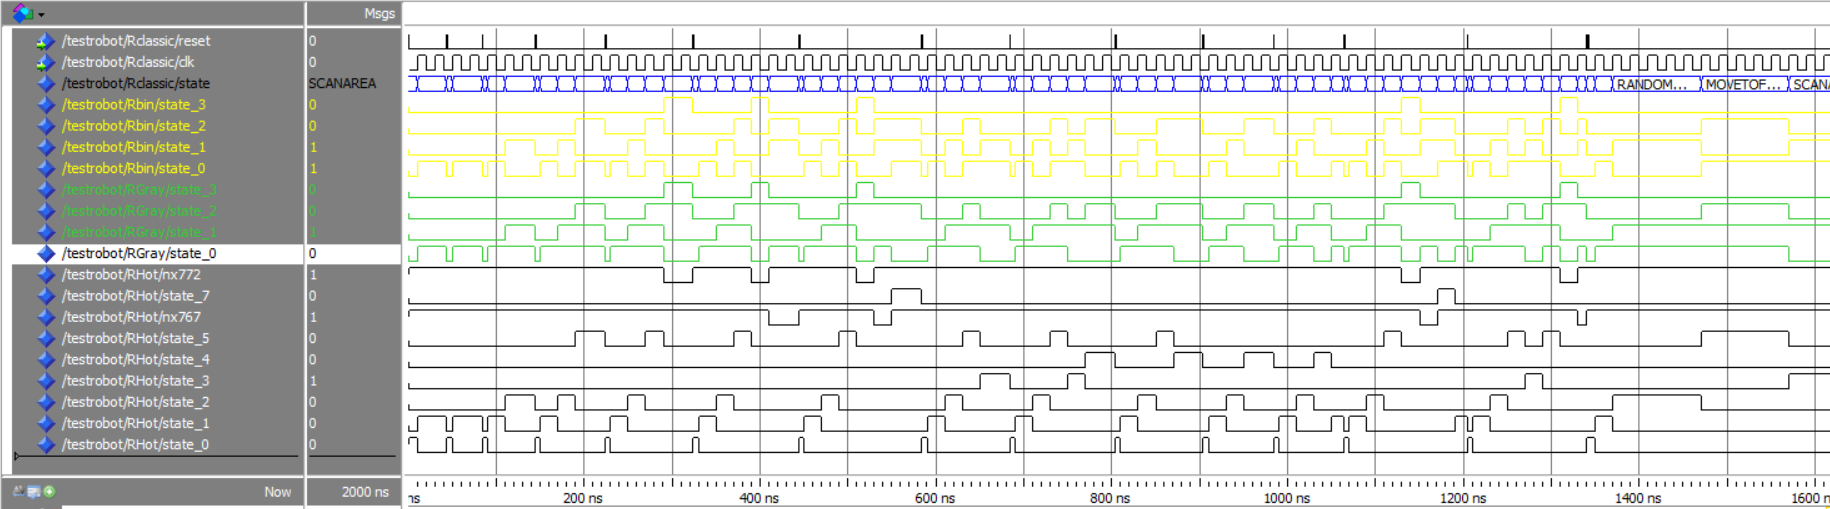
\includegraphics[scale=0.6]{C/CLEAN.PNG}
\caption{Chronograme avec les signaux d'états }
\end{figure} 

Ce qui correspond bien avec ce qui était attendu.

\end{landscape}


En faisant un montage on peux alors vérifier plus simplement toutes les valeurs pour chaque états.

\begin{figure}[!h]
\centering
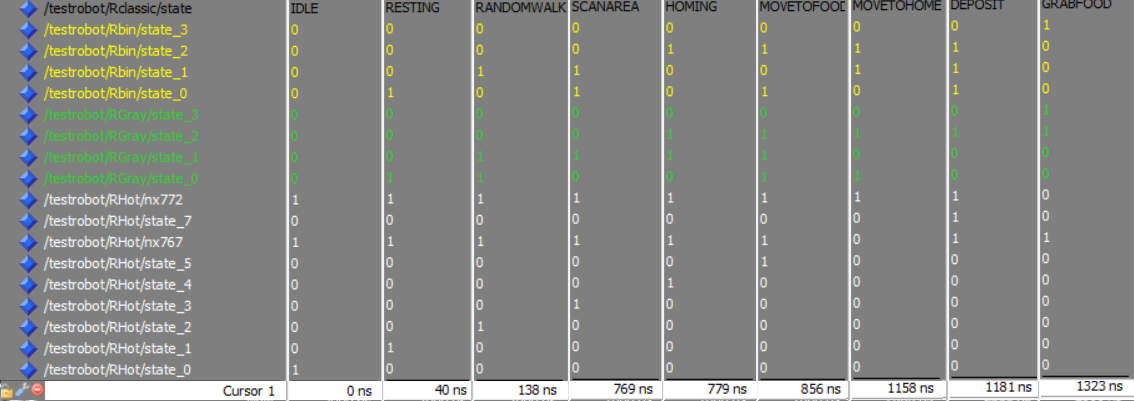
\includegraphics[scale=0.6]{C/STATE.PNG}
\caption{Montage du chronograme avec les différentes valeurs de sorties }

Il est aussi possible de créer des propriété PSL verifiant les valeurs des signaux des synthèses en fonction de la valeur de l'état sur le système non synthétisé.
\end{figure} 

\section{Assertion}

Pour vérifier que les assertions temporelles définies au TP précédent restent satisfaite après synthèse il faut réecrire les assertions dans les fichiers de synthèse et remplacer les endroits où l'on test la valeur d'un état par son identité en encodage. Voix annexes.

Pour vérifier que les nouvelles assertions soient juste il suffit de les regrouper et de vérifier qu'elles sont identique comme suit :

\begin{figure}[!h]
\centering
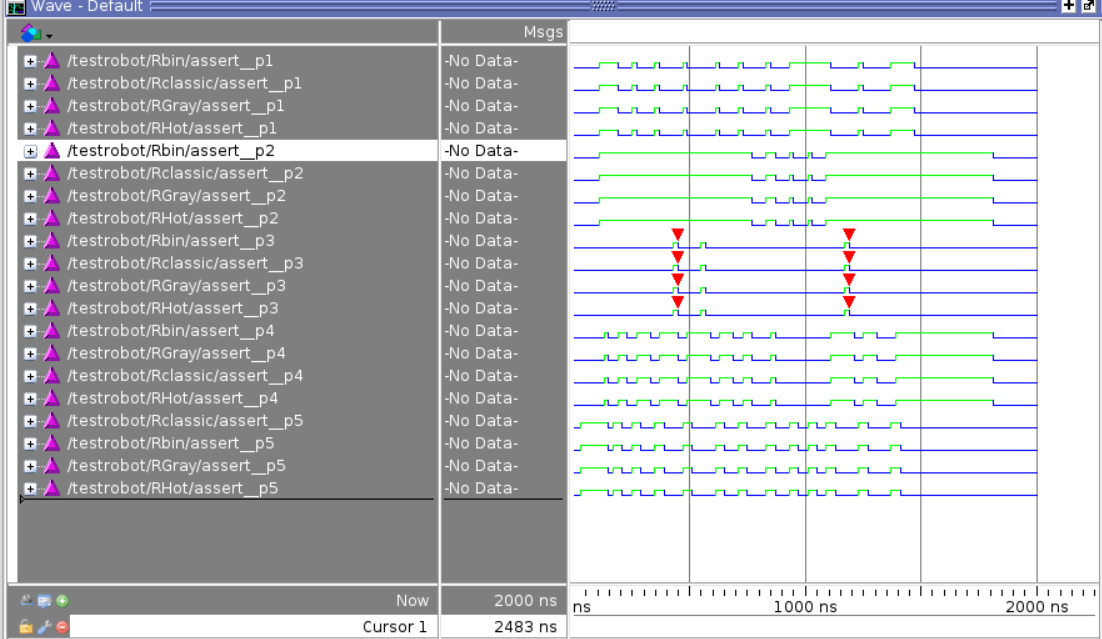
\includegraphics[scale=0.6]{D/testFULL.PNG}
\caption{Assertions P1, P2, P3, P4 et P5 sur le chronogramme }
\end{figure}

Pour vérifier que les sorties des architectures soient toujours identique j'ai crée trois assertions qui vérifie ceux-ci grace à une formule booléenne :

\begin{verbatim}
-- psl property RestAlwaysTheSame is always ( ((re = '0' or reBin = '0' or reGray = '0' or reHot = '0') 
	-- AND (re = '0' and reBin = '0' and reGray = '0' and reHot = '0' and testPSL = '0'))
	-- OR  ((re = '1' or reBin = '1' or reGray = '1' or reHot = '1') AND (re = '1' and reBin = '1' and reGray = '1' and reHot = '1')) );
	-- psl assert RestAlwaysTheSame;
\end{verbatim}

\begin{figure}[!h]
\centering
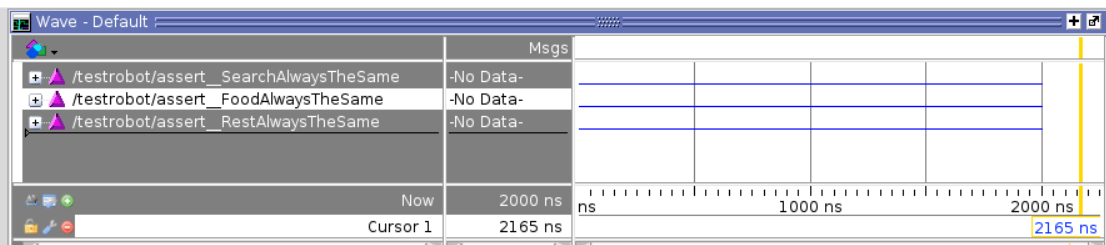
\includegraphics[scale=0.6]{D/testOK.PNG}
\caption{Assertion verifiant l'égalité des sorties}
\end{figure}
Aucune assertion échoue donc sela semble fonctionner.
Pour vérifier on rajoute un signal qui est toujours égale à 1 dans une des clauses et on obtiens :

\begin{figure}[!h]
\centering
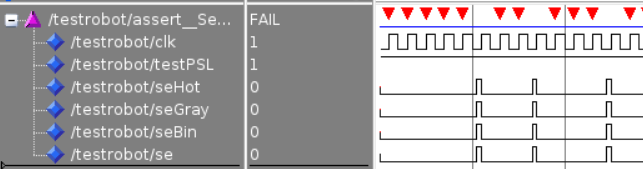
\includegraphics[scale=0.6]{D/testFAIL.PNG}
\caption{Test de l'assertion verifiant l'égalité des sorties }
\end{figure}
Les formules sont donc juste.
\newpage

\section{Synthèse du compteur}
\subsection{Compteur non borné}
D'après les résultats obtenus après synthèse (voir annexes). Il y a 31 DFC1 et 1 DFCP1 soit un total de 32 flip flops. Il y a en tout 32 flips flops parce que notre signal peut être codé sur 32 bits. Il faut alors de quoi stocker ses 32 bits.

La surface obtenue est 17963 um2 

La fréquence obtenue est 155.2 MHz


\subsection{Compteur avec valeur borné}

D'après les résultats obtenus après synthèse (voir annexes). Il y a 4 DFC1 et 1 DFCP1 soit un total de 5 flip flops. Il y a en tout 5 flips ce qui parrait étrange car $log_2(10) = 3.3 $, 4 flips flops aurais suffit. 

La surface obtenue est  2639 um2 

La fréquence obtenue est  685.2 MHz

\subsection{Conclusion}

Nous travaillons ici dans un système où chaque choix de design aura un impact sur la synthèse du système : la surface a était réduit plus de 6 fois est la fréquence à plus que quadruplé. Il faut donc bien faire attention car l'erreur est beaucoup plus vite punitive habituellement. Il font donc faire preuve de rigueur.

\newpage
\section{Annexes}
\subsection{Descprition comportementale du système de contrôle}
\subsubsection{Premier process}
\subsubsubsection{Code VHDL}

\begin{verbatim}
process (state, athome, findfood, lostfood, closetofood, success,
 aboverestth, abovesearchth, scantimeup)
	begin
		case state is
			when IDLE => nextstate <= RESTING;
			when RESTING => 
				if aboverestth = '1' then nextstate <= RANDOMWALK;
				else--elsif aboverestth = '0' then 
				nextstate <= RESTING;
				end if;
				
			when RANDOMWALK => 
				if abovesearchth = '1' then nextstate <= HOMING;
				else--  abovesearchth = '0' then
					if findfood = '1' then nextstate <= MOVETOFOOD;
					else--elsif findfood = '0' then
						nextstate <= RANDOMWALK;
					end if;
				end if;
				
			when SCANAREA => 
				if abovesearchth = '1' then nextstate <= HOMING;
				else--elsif  abovesearchth = '0' then
					if findfood = '1' then nextstate <= MOVETOFOOD;
					else--elsif findfood = '0' then
						if scantimeup = '1' then nextstate <= RANDOMWALK;
						else--elsif scantimeup = '0' then 
						nextstate <= SCANAREA; 
						end if;
					end if;
				end if;
			when HOMING => if(athome = '1') then nextstate <= RESTING; else nextstate <= HOMING; end if;
			when MOVETOFOOD => 
				if abovesearchth = '1' then nextstate <= HOMING;
				else--elsif  abovesearchth = '0' then
					if lostfood = '1' then nextstate <= SCANAREA;
					else--elsif lostfood = '0' then
						if closetofood = '1' then nextstate <= GRABFOOD;
						else--elsif closetofood = '0' then
							nextstate <= MOVETOFOOD; 
						end if;
					end if;
				end if;
			when GRABFOOD =>
				if success = '1' then nextstate <= MOVETOHOME;
				else--elsif success = '0' then
				 nextstate <= GRABFOOD;
				end if;
			when MOVETOHOME =>
				if athome = '1' then nextstate <= DEPOSIT;
				else--elsif athome = '0' then
				 nextstate <= MOVETOHOME;
				end if;
			when DEPOSIT =>
				if success = '1' then nextstate <= RESTING;
				else--elsif success = '0' then
				 nextstate <= DEPOSIT;
				end if;
		end case;
	end process;
\end{verbatim}

\subsubsubsection{Bloc combinatoire ou mémorisant}

"The VHDL process that characterizes the next state generation corresponds to the transition function
combinational block:"

Alors c'est un bloc combinatoire
\subsubsubsection{Liste de sensibilité}

Tout ce qui peux alors modifier la valeur du prochain état Soit tout ce qui se trouve dans les branchements. 

\subsubsubsection{Composants utilisé}
Ce sera alors des composants combinatoires qui seront utilisé


\newpage
\subsubsection{Second process}
\subsubsubsection{Code VHDL}
\begin{verbatim}
	process(reset, clk)
	begin
		-- RESET : asynchrone haut
		if reset = '1' then state <= IDLE;
		-- HORLOGE : front montant 
		elsif (clk'event and clk = '1') then
			state <= nextstate;
		end if;
	end process;
\end{verbatim}


\subsubsubsection{Bloc combinatoire ou mémorisant}
"And the "clocked process" expresses the updating of the flip-flops (registers)"

C'est un bloc mémorisant

\subsubsubsection{Liste de sensibilité}
L'horloge et le reset

\subsubsubsection{Composants utilisé}

Des composants mémorisants

\newpage
\subsubsection{Output process}
Mon process d'output est en fait plusieurs affectations représentant les process. Cela permet une optimisation car la liste de senssibilité est réduite.
\subsubsubsection{Code VHDL}
\begin{verbatim}
rest <= '1' when (( state = DEPOSIT and success = '1' ) OR (state = IDLE) OR (state = HOMING and
     athome = '1') ) else '0';
search <= '1' when (state = RESTING and aboverestth = '1' ) else '0';
food <= '1' when  (state = MOVETOFOOD and abovesearchth = '0' and lostfood = '0' and closetofood ='1')
    else '0';
\end{verbatim}
\subsubsubsection{Bloc combinatoire ou mémorisant}
"The VHDL process that characterizes the output generation corresponds to the output function combinational block:"

Bloc combinatoire
\subsubsubsection{Liste de sensibilité}
Chaque outputs possède sa propre liste de sensibilité qui est les différents items utilisé dans la formule.
\subsubsubsection{Composants utilisé}
Ce sera alors des composants combinatoires qui seront utilisé

\newpage
\subsection{Descprition comportementale du compteur}
J'ai modifié le compteur pour qu'il ne soit plus générique tel que 
\begin{verbatim}
Signal threshold : natural = 4;
\end{verbatim}
\subsubsection{Premier process}
\subsubsubsection{Code VHDL}
	process (state, start, c)
	begin
		case state is
		when IDLE =>
			if start = '1' then 
				nextstate <= COUNTING; 
			elsif start = '0' then
				nextstate <= IDLE;
			end if;
		when COUNTING =>
			if c < threshold then	
				nextstate <= COUNTING;
			else 
				nextstate <= IDLE;
			end if;
		end case;
	end process;
\subsubsubsection{Bloc combinatoire ou mémorisant}
Combinatoire
\subsubsubsection{Liste de senssibilité}
state, start, c
\subsubsubsection{Composants utilisé}
Combinatoire
\newpage
\subsubsection{Deuxième process}
\subsubsubsection{Code VHDL}
process(reset, clk, start)
	begin
		-- RESET : asynchrone haut
		if reset = '1' then 
			state <= IDLE;
		-- HORLOGE : front montant 
		elsif ( (start = '1') and (state = IDLE) )then
				state <= COUNTING;
				
		elsif (clk'event and clk = '1') then
			state <= nextstate;
		-- Detecter un pic sur start
	
		end if;
		
		
	end process;
\subsubsubsection{Bloc combinatoire ou mémorisant}
Mémorisant
\subsubsubsection{Liste de senssibilité}
reset, clk, start
\subsubsubsection{Composants utilisé}
Mémorisant et combinatoire

\newpage
\subsubsection{Troisième process}
\subsubsubsection{Code VHDL}
process(start, clk, reset)
	begin
		if(reset = '1') then
			c <= 0;
			
		else 
			if (clk'event and clk = '1') then
				if (state = IDLE and start = '0') then 
					C <= 0;
				elsif ( state = IDLE and start = '1') then
					c <= c + 1;
				elsif (state = COUNTING and c < threshold) then
					c <= c + 1;
				elsif(state = COUNTING and c >= threshold) then
					c <= 0;
				end if;
			end if;
		end if;
	end process;
\subsubsubsection{Bloc combinatoire ou mémorisant}
Mémorisant (valeur du compteur)
\subsubsubsection{Liste de senssibilité}
start, clk, reset
\subsubsubsection{Composants utilisé}
Combinatoire et mémorisant
\newpage
\subsubsection{Quatrième process}
\subsubsubsection{Code VHDL}
process(c)
	begin
		if  (c >= threshold) then
			aboveth <= '1';
		else aboveth <= '0';
		end if;
	end process;
\subsubsubsection{Bloc combinatoire ou mémorisant}
Combinatoire
\subsubsubsection{Liste de sensibilité}
Valeur du compteur
\subsubsubsection{Composants utilisé}
Combinatoires

\newpage
\subsection{Synthèse du contrôleur}

\subsubsection{Encodage binaire}
\subsubsubsection{Codage des états}
\begin{verbatim}

\end{verbatim}
\subsubsubsection{Report Area}
\begin{verbatim}

\end{verbatim}
\subsubsubsection{Report Delay}
\begin{verbatim}

\end{verbatim}

\newpage
\subsubsection{Encodage de Gray}
\subsubsubsection{Codage des états}
\begin{verbatim}

\end{verbatim}
\subsubsubsection{Report Area}
\begin{verbatim}

\end{verbatim}
\subsubsubsection{Report Delay}
\begin{verbatim}

\end{verbatim}

\newpage
\subsubsection{Encodage OneHot}
\subsubsubsection{Codage des états}
\begin{verbatim}

\end{verbatim}
\subsubsubsection{Report Area}
\begin{verbatim}

\end{verbatim}
\subsubsubsection{Report Delay}
\begin{verbatim}

\end{verbatim}

\newpage
\subsection{Synthèse du compteur}
\subsubsection{Sans borner C}
\subsubsubsection{Report Area}
\begin{verbatim}

\end{verbatim}
\subsubsubsection{Report Delay}
\begin{verbatim}
\end{verbatim}

\subsubsection{Avec C borné}

\subsubsubsection{Report Area}
\begin{verbatim}

\end{verbatim}
\subsubsubsection{Report Delay}
\begin{verbatim}
\end{verbatim}

\end{document}